\documentclass[notitlepage]{revtex4-2}

\usepackage{graphicx}
\usepackage{amsmath}
\usepackage{bm}
\usepackage{bbold}
\usepackage{xcolor}
\usepackage{cancel}
\renewcommand{\CancelColor}{\color{red}}
\begin{document}
\title{Doc: continuous models}
\author{Laurent Pagnier and Julian Fritzsch}
\maketitle

\begin{equation}
m(\bm x)\frac{\partial^2}{\partial t^2}\theta(\bm x,t)+d(\bm x)\frac{\partial}{\partial t}\theta(\bm x,t)=p(\bm x,t)+\bm\nabla\cdot\big[\bm b(\bm x)\circ\bm\nabla\theta(\bm x,t)\big]\,,
\end{equation}
Discretizing in time and space, updated state is computed as 
\begin{align}
\theta_{i,j}(t+\Delta t) &= 
\bigg[2\chi_{ij} -\frac{\Delta t^2 m_{ij}^{-1}\chi_{ij}}{\Delta x^2}\Big(b_{i,j|i+1,j}+b_{i-1,j|i,j}+b_{i,j|i,j+1}+b_{i,j-1|i,j}\Big)\bigg]\theta_{i,j}(t)\nonumber\\
&-\Big[1-\frac{\gamma_{i,j}\Delta t}{2}\Big]\chi_{ij}\theta_{i,j}(t-\Delta t) +\frac{\Delta t^2 \chi_{i,j}m_{ij}^{-1}}{\Delta x^2}\bigg[b_{i-1,j|i,j}\theta_{i-1,j}(t)+b_{i,j|i+1,j}\theta_{i+1,j}(t)\nonumber\\
&+b_{i,j-1|i,j}\theta_{i,j-1}(t)
+b_{i,j|i,j+1}\theta_{i,j+1}(t)\bigg] + \Delta t^2 \chi_{ij} m_{ij}^{-1}p_{i,j}\,,
\end{align}
where $\chi_{i,j}=\Big[1+\frac{\gamma_{i,j}\Delta t}{2}\Big]^{-1}$ and $\gamma_{i,j}=d_{i,j}/m_{i,j}$.

The previous equation follows from
\begin{equation}
\bm\nabla\cdot\big[\bm b(\bm x)\circ\bm\nabla\theta(\bm x,t)\big]=\partial_xb_x\partial_x\theta+b_x\partial_x^2\theta +\partial_yb_y\partial_y\theta+b_y\partial_y^2\theta\,,
\end{equation}
where
\begin{align}
b_x(\bm x)&\approx\frac{b^x_{i,j-1}+b^x_{i,j}}{2}\,,\\
\partial_xb_x&\approx\frac{b^x_{i,j}-b^x_{i,j-1}}{\Delta x}\,,\\
\partial_x\theta&\approx\frac{\theta_{i+1,j}-\theta_{i-1,j}}{2\Delta x}\,,\\
\partial_x^2\theta&\approx\frac{\theta_{i-1,j}-2\theta_{i,j}+\theta_{i+1,j}}{\Delta x^2}\,,
\end{align}
So, finally
\begin{align}
&\partial_xb_x\partial_x\theta+b_x\partial_x^2\theta +\partial_yb_y\partial_y\theta+b_y\partial_y^2\theta\approx\\
&\frac{b^x_{i,j-1}\theta_{i,j-1}+b^x_{i,j}\theta_{i,j+1}+b^y_{i-1,j}\theta_{i-1,j}+b^y_{i,j}\theta_{i+1,j}-\overbrace{\big(b^x_{i,j-1}+b^x_{i,j}+ b^x_{i-1,j}+b^y_{i,j}\big)}^{=\beta}\theta_{i,j}}{\Delta x^2}\,,
\end{align}
\section{Steady State}
Steady state is obtained iteratively as
\begin{align}
\theta_{i,j}^{(n+1)} &= \frac{\Delta x^2\,p_{i,j} + b^y_{i,j}\theta_{i-1,j}^{(n)}
%%
+b^y_{i,j}\theta_{i+1,j}^{(n)}+b^x_{i,j-1}\theta_{i,j-1}^{(n)}
+b^x_{i,j}\theta_{i,j+1}^{(n)}}
%%
{b^y_{i,j}+b^y_{i-1,j}+b^x_{i,j}+b^x_{i,j-1}}
\end{align}


\begin{figure}
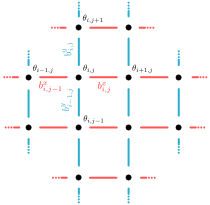
\includegraphics[width=0.5\textwidth]{figures/lattice_implementation.pdf}
\caption{How it is implemented.}
\end{figure}

\section{Boundary conditions}
\begin{equation}
\intop_{\partial \Omega}b(\bm x)\circ\nabla \theta(\bm x,t)\cdot\bm n\, {\rm d}\bm x  = 0 \\,
\end{equation}
which is trivially true, if
\begin{equation}
n_xb_x\partial_x \theta(\bm x) + n_yb_y\partial_y \theta(\bm x) = 0\,,\; \forall t \text{ and } \bm x \in \partial \Omega \,,
\end{equation}
For the moment, lets assume in 1D and treating the case $n_x=-1$.
\begin{equation}
b_x(x)\partial_x \theta(x) = 0
\end{equation}

\begin{align}
b_x(x+\Delta x)\theta(x+\Delta x) &= b_x(x)\theta(x) + \Big(\partial_x b_x(x) \theta(x)+ \cancelto{0,\text{ b.c.}}{b_x(x)\partial_x \theta(x)}\Big)\Delta x + (\cdots)\Delta x^2/2 + O(\Delta x^3)\\
b_x(x+2\Delta x)\theta(x+2\Delta x) &= b_x(x)\theta(x) + \Big(\partial_x b_x(x)\theta(x)+ \cancelto{0,\text{ b.c.}}{b_x(x)\partial_x \theta(x)}\Big)2\Delta x + 2(\cdots)\Delta x^2 + O(\Delta x^3)
\end{align}
(From the 1st equation, we get
\begin{equation}
\theta_{i,j}=\frac{(b^x_{i,j}+b^x_{i,j+1})\theta_{i,j+1}}{3 b^x_{i,j} {\color{red}- b^x_{i,j-1}}}+O(\Delta x^2)
\end{equation}
which is not exactly what was implemented. It might be enough to change that...)
Summing four times the 1st equation with minus the second, one gets
\begin{equation}
\theta(x) = \frac{4b_x(x+\Delta x)\theta(x+\Delta x)-b_x(x+2\Delta x)\theta(x+2\Delta x)}{3b_x(x)+2\Delta x\partial_xb_x}+O(\Delta x^3)
\end{equation}
Converting this expression with Eqs. 4-7, we get
\begin{equation}\label{eq:thetanx}
\theta_{i,j} = \frac{4(b^x_{i,j}+b^x_{i,j+1})\theta_{i,j+1} - (b^x_{i,j+1}+b^x_{i,j+2})\theta_{i,j+2}}{3(b^x_{i,j-1}+b^x_{i,j})+4(b^x_{i,j}-b^x_{i,j-1})}
\end{equation}
What to do? Set $b^x_{i,j-1}$ to $0$ or to $b^x_{i,j}$!? (My opinion is that we should set it to 0. {\color{red}I agree with that.})

{\color{red}Analogously we obtain for $n_x=1$ we obtain by changing $\Delta x \to - \Delta x$
\begin{equation}
    \theta_{i,j}=\frac{4(b^x_{i,j-2}+b^x_{i,j-1})\theta_{i,j-1}-(b^x_{i,j-3}+b^x_{i,j-2})\theta_{i,j-2}}{3(b^x_{i,j-1}+b^x_{i,j})-4(b^x_{i,j}-b^x_{i,j-1})}
\end{equation}
In this case we should set $b^x_{i,j}=0$.

For the corners we can use ($n_x=-1$, $n_y=-1$)
\begin{align}
    \begin{split}
    &b_x(x+\Delta, y)\theta(x+\Delta, y) + b_y(x, y + \Delta)\theta(x, y+ \Delta) = (b_x(x,y) + b_y(x,y))\theta(x,y) + \\
    &\big(b_x(x,y)\cancelto{0, b.c.}{\partial_x\theta(x,y) + b_y(x,y)\partial_y\theta(x,y)} + b_x(x,y)\partial_y\theta(x,y) + b_y(x,y)\partial_x\theta(x,y)\big)\Delta + (\dots)\Delta^2/2 + \mathcal{O}(\Delta^3),
    \end{split}\\
    \begin{split}
        &b_x(x+2\Delta, y)\theta(x+2\Delta, y) + b_y(x, y + 2\Delta)\theta(x, y+ 2\Delta) = (b_x(x,y) + b_y(x,y))\theta(x,y) + \\
        &2\big(b_x(x,y)\cancelto{0, b.c.}{\partial_x\theta(x,y) + b_y(x,y)\partial_y\theta(x,y)} + b_x(x,y)\partial_y\theta(x,y) + b_y(x,y)\partial_x\theta(x,y)\big)\Delta + 2(\dots)\Delta^2 + \mathcal{O}(\Delta^3)
        \end{split}
\end{align}
This means for the corners the $\theta_{i,j}$ is given by the sum of~\eqref{eq:thetanx} and its $y$ equivalent.}

Now treating the full case {\color{red}(setting the $b$ outside the grid to 0)}, lets first define 
\begin{equation}
\eta_{\pm}(x) = 1\pm x/2 -x^2/2\,,
\end{equation}
Note that $\eta_{+}(-1)=0$, $\eta_{+}(0)=1$, $\eta_{+}(1)=1$, $\eta_{-}(-1)=1$, $\eta_{-}(0)=1$ and $\eta_{-}(1)=0$.
\begin{equation}
\beta=\eta_{+}(n_x)b^x_{i,j-1}+\eta_{-}(n_x)b^x_{i,j}+\eta_{+}(n_y)b^y_{i,j-1}+\eta_{-}(n_y)b^y_{i,j}\,,
\end{equation}




\section{Vectorization}
The different quantities are flattened, as follows
\begin{equation}
\theta_{i,j} \rightarrow \tilde\theta_k\,,
\end{equation}
with $k = N_y(i-1)+j$. With this change in the indexing, the indices of neighbouring nodes become
\begin{align}
i-1,j &\rightarrow k-1\,,\\
i+1,j &\rightarrow k+1\,,\\
i,j-1 &\rightarrow k-N_y\,,\\
i,j+1 &\rightarrow k+N_y\,,
\end{align}

\begin{equation}
\xi_{i,j}(\bm \theta)=-\big(b^x_{i,j-1}+b^x_{i,j}+b^y_{i-1,j}+b^y_{i,j}\big)\theta_{i,j}
%%
+b^x_{i,j-1}\theta_{i,j-1}
%%
+b^x_{i,j}\theta_{i,j+1}
%%
+b^y_{i-1,j}\theta_{i-1,j}
%%
+b^y_{i,j}\theta_{i+1,j}\,,
\end{equation}
The function $\bm \xi(\bm \theta)$ can be represented as a matrix acting on the flattened $\bm{\tilde \theta}$,
\begin{equation}
\bm \xi(\bm \theta) =\bm \Xi\, \bm{\tilde\theta}\,.
\end{equation}
The elements of $\bm \Xi$ read
\begin{equation}
\Xi_{kl} = -\big(\tilde b^x_{k}+\tilde b^x_{k-N_y}+\tilde b^y_{k}+\tilde b^y_{k-1}\big)\delta_{k,l}
%%
+\tilde b^{x}_{k-N_y}\delta_{k-N_y,l}
%%
+\tilde b^{x}_{k}\delta_{k+N_y,l}
%%
+\tilde b^{y}_{k-1}\delta_{k-1,l}
%%
+\tilde b^{y}_{k}\delta_{k+1,l}\,,
\end{equation}
with $\delta_{\cdot,\cdot}$ is the Kronecker product.
\section{Crank–Nicolson}

\begin{equation}
 \theta_{i,j}(t+\Delta t) -\frac{\Delta t}{2}\,\omega_{i,j}(t+\Delta t) = \theta_{i,j}(t) + \frac{\Delta t}{2}\,\omega_{i,j}(t)\,,
\end{equation}

\begin{equation}
\Big(1+\frac{\gamma_{i,j}\Delta t}{2}\Big)\omega_{i,j}(t+\Delta t) - \frac{\Delta t}{2}\xi\big(\theta_{i,j}(t+\Delta t)\big)
%%
=
%%
\Big(1-\frac{\gamma_{i,j}\Delta t}{2}\Big)\omega_{i,j}(t)+\frac{\Delta t}{2}\xi\big(\theta_{i,j}(t)\big) + (2m_{i,j})^{-1}\Big[p_{i,j}(t+\Delta t) + p_{i,j}(t)\Big]\,,
\end{equation}

\begin{equation}
\underbrace{\left[\begin{array}{cc}
\mathbb{1} & -\frac{\Delta t}{2} \mathbb{1}\\
-\frac{\Delta t}{2\Delta x^2}\,\bm M^{-1}\,\bm \Xi & \mathbb{1} + \frac{\Delta t}{2}\,\bm\Gamma
\end{array}\right]}_{=\bm A}\bm x(t+ \Delta t)
%%
=
%%
\underbrace{\left[\begin{array}{cc}
\mathbb{1} & \frac{\Delta t}{2} \mathbb{1}\\
\frac{\Delta t}{2\Delta x^2}\,\bm M^{-1}\,\bm \Xi & \mathbb{1} - \frac{\Delta t}{2}\,\bm\Gamma
\end{array}\right]}_{=\bm B}\bm x(t) +
%%
\underbrace{ \left[\begin{array}{c}
\mathbb{0}\\
\bm \pi\end{array}\right]}_{=\bm C}\,,
\end{equation}
with $\bm x^\top = [\bm{\tilde \theta}^\top\; \bm{\tilde \omega}^\top]$.


\section{Higher orders}

\begin{equation}
\partial_x^2\theta = \frac{-\theta_{i,j-2}+16\,\theta_{i,j-1}-30\,\theta_{i,j}+16\,\theta_{i,j+1}-\theta_{i,j+2}}{24\Delta x^2}+O(\Delta x^5)\,,
\end{equation}
\begin{equation}
\partial_x\theta = \frac{\theta_{i,j-2}-8\,\theta_{i,j-1}+8\,\theta_{i,j+1}-\theta_{i,j+2}}{12\Delta x}+O(\Delta x^5)\,,
\end{equation}
\begin{equation}
\partial_x b_x = \frac{b^x_{i,j-2}-27\,b^x_{i,j-1}+27\,b^x_{i,j}-b^x_{i,j+1}}{48\Delta x}+O(\Delta x^5)\,,
\end{equation}

\begin{align}
\partial_xb_x\partial_x\theta_x + b_x\partial_x^2\theta &=
%%
\Big[(b^x_{i,j-2}-29\,b^x_{i,j-1}+25\,b^x_{i,j}-b^x_{i,j+1})\theta_{i,j-2}\\
%%
&+(b^x_{i,j-2}-152\,b^x_{i,j-1}+280\,b^x_{i,j}-b^x_{i,j+1})\theta_{i,j-1}\\
%%
&-(48b^x_{i,j-1}+48b^x_{i,j})\theta_{i,j}\Big]/ (576\Delta x^2) (FALSE TODO)
\end{align}
\end{document}
